% CO1 — AI Workforce Odyssey (Coding) — Short memo
% Compile with: pdflatex memo.tex (twice if references/cross-refs added)
% Replace figure paths with your exported screenshots from NetLogo.

\documentclass[11pt,letterpaper]{article}

\usepackage[margin=1in]{geometry}
\usepackage{graphicx}
\usepackage{booktabs}
\usepackage{hyperref}
\usepackage{enumitem}
\usepackage{parskip}

\hypersetup{
  colorlinks=true,
  linkcolor=blue,
  urlcolor=blue,
  pdftitle={AI Workforce Odyssey: Brigade Staff ABM Memo},
  pdfauthor={Ariana Rocha}
}

\title{\textbf{AI Workforce Odyssey: Agent-Based Simulation}\\[0.35em]
\large Brigade Staff Workforce Dynamics Under AI-Oriented Pressure}
\author{Ariana Rocha (afrocha)\\
Agentic Technologies: Individual Assignment \#1 (Coding)}
\date{March 22, 2026}

\begin{document}
\maketitle

\begin{abstract}
This memo describes a compact NetLogo~7 agent-based model of thirty workers arranged in a deployed brigade staff environment. Workers differ in task profile, position, resilience, and an \emph{AI disruption risk} index. Policy-level choices appear as \emph{scenario parameters}, not as separate agent classes. The model compares \textbf{Tech-Driven Automation} and \textbf{Human-Centric Support}. Programmed rules govern timed training, probabilistic movement to at-risk status, training uptake, casualties, and load redistribution. An emergent pattern arises from \textbf{load pooling across survivors}, which couples workload and burnout as headcount falls. Outputs include mission capability, combat power, average load, and burnout over a fixed deployment horizon.
\end{abstract}

% ---------------------------------------------------------------------------
\section{Model Overview (Defining the World)}

This model treats a deployed brigade headquarters (BDE HQ) as a compact labor market under AI transition pressure: each staff member is a worker, each shop function is a task domain, and attempted AI integration into planning, reporting, and decision support is the disruption source. The framing allows the assignment’s workforce concepts to map directly onto an operational setting: workers differ in task profile, resilience/adaptability, and disruption risk; they move through explicit states (employed, at-risk, in-training, re-employed, unemployed/casualty); and repeated local interactions generate system-level effects. In particular, staffing losses and training bottlenecks redistribute work, which can amplify burnout over time and create unequal recovery patterns across the force. The result is a small but explainable model that supports comparisons between Tech-Driven Automation and Human-Centric Support using the same underlying structure.

The world is intentionally simple: \textbf{30 agents} (\texttt{soldiers}) occupy a \textbf{$5 \times 6$} lattice representing \textbf{five shift bands} and \textbf{six staff shops} (including command). Each tick represents one \textbf{week} of a \textbf{36-week} deployment. The visualization encodes \textbf{workforce state} by color (training, employed, at-risk, re-employed, unemployed/casualty), with a lower \textbf{casualty band} labeled for casualty collection: Killed in Action (KIA), Wounded In Action (WIA), and Out of Fight (OOF) for readability.

\textbf{Scenario} is selected via an Interface chooser and implemented through \texttt{apply-scenario-presets}: \textbf{Tech-Driven Automation} uses higher \textbf{automation pressure}, tighter human-loop coupling to automation, higher training-seat pressure (harder access to remediation), direct kill-chain AI, and faster growth of a global \textbf{AI system capability} score. \textbf{Human-Centric Support} lowers automation pressure, strengthens human-loop effect, eases training-seat pressure, disables the direct kill-chain flag, starts from a lower AI capability baseline, and caps AI growth more conservatively. Optional Interface sliders (\textbf{casualty-risk-level}, \textbf{burnout-sensitivity}) scale stochastic casualties and burnout dynamics for sensitivity analysis; they are not separate agents.

% --- Figure: replace path with your screenshot ---
\begin{figure}[htbp]
  \centering
  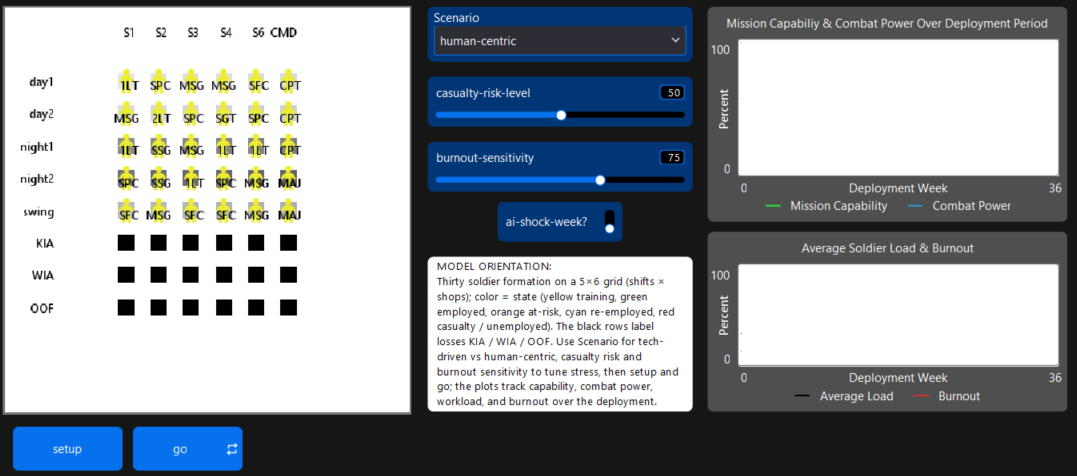
\includegraphics[width=0.92\textwidth]{model_snip0.png}
  \caption{NetLogo Interface: formation grid (5 shifts $\times$ 6 shops: S1 Personnel, S2 Intelligence, S3 Operations, S4 Logistics, S6 Signal, and CMD), scenario controls, and system-level outputs over weeks. In this setup, disruption pressure is generally higher in S1/S2/S4 and lower in S3/S6/CMD.}
  \label{fig:interface}
\end{figure}

% ---------------------------------------------------------------------------
\section{Soldier Profile (Worker Attributes)}

Each worker carries attributes aligned with the assignment rubric:

\begin{itemize}[leftmargin=*]
  \item \textbf{Task profile / task mix:} Military Occupational Specialty (MOS) code, plus \textbf{shop} and \textbf{position} (e.g., S2 Intelligence, S6 Signal). A routine score derived from MOS feeds into AI disruption.
  \item \textbf{Behavioral trait:} \textbf{Resilience} (with competence as a secondary factor) governs how quickly burnout rises under workload and how heavy baseline assignments feel; in this model, \textbf{rank} is used as a practical proxy for resilience/adaptability on average, with the caveat that adaptation varies across individuals at every rank and recognizing there is a case to be made about younger soldiers being more adaptable to AI disruptions.
  \item \textbf{AI disruption risk:} Turtle variable \textbf{\texttt{disruption-risk}} (bounded), computed from MOS routine, position-based modifiers (e.g., signal, intel, command), and stochastic noise at initialization. It scales the probability of transitioning from \textbf{employed/re-employed} to \textbf{at-risk} together with scenario-level \textbf{automation pressure} and \textbf{human-loop effect}.
  \item \textbf{Current state:} \texttt{state-name} $\in$ \{\texttt{in-training}, \texttt{employed}, \texttt{at-risk}, \texttt{re-employed}, \texttt{unemployed}\}.
\end{itemize}

% ---------------------------------------------------------------------------
\section{Soldier Status (Worker States and Programmed Transitions)}

\section{Worker States and Programmed Transitions}

Worker states are explicitly programmed and update once per weekly tick. The initial \texttt{setup} places all personnel in \texttt{in-training} with staggered time offsets to simulate rolling arrivals into country.

\begin{itemize}[leftmargin=*]
  \item \textbf{Timed transition rule (training completion):} if \texttt{training-ticks-left} reaches zero, workers exit training. Initial training produces employed status; AI-week remediation produces re-employed status. This is an elapsed-time rule.
  \item \textbf{Probabilistic disruption rule (employed/re-employed to at-risk):} non-command workers move to at-risk with probability driven by automation pressure, personal disruption risk, and human-loop effect. Higher disruption-risk workers under tech-driven settings are more likely to transition.
  \item \textbf{Condition-based recovery rule (at-risk to in-training):} at-risk workers can enter short AI-week retraining, with access constrained by scenario-level training-seat pressure. This creates explicit support differences across scenarios.
  \item \textbf{Probabilistic casualty rule (active states to unemployed):} workers in active states face a contact-style casualty draw each week, then are classified as KIA, WIA, or OOF for display since in combat someone is only ever``unemployed" if they are a casualty.
\end{itemize}

Together, these rules satisfy the assignment requirement for multiple explicit transition types (timed, probabilistic, and condition-constrained) while keeping the model small and readable.

% ---------------------------------------------------------------------------
\section{Emergent Mechanism}

The assignment asks for at least one interaction mechanism that produces a \textbf{system-level pattern} from local rules. This model emphasizes a \textbf{training and load bottleneck with redistribution}:

\begin{itemize}[leftmargin=*]
  \item When some workers are in \textbf{AI-focused retraining} (\texttt{in-training} with a short tick counter), the count of soldiers operating drops relative to total surviving staff.
  \item \textbf{\texttt{redistribute-load-and-burnout}} reallocates workload across employed, at-risk, and re-employed agents as a function of the \textbf{share in training} and scenario flags. That creates \textbf{peer-conditional load spillover}: the same global staffing task is carried by fewer fully-available people, so mean workload and burnout can rise even when individual ``productivity'' rules are unchanged.
  \item \textbf{Casualties} further shrink the survivor pool; reported \textbf{average load} can incorporate a \textbf{carry factor} (fewer survivors $\Rightarrow$ higher effective burden per living agent) and stronger coupling to mean survivor burnout, so the load and burnout time series \textbf{co-move} with headcount losses, a pattern that is not hard-coded as a single global equation but arises from repeated micro-updates.
\end{itemize}

% ---------------------------------------------------------------------------
\section{Scenario Results with Outputs}

\textbf{Tech-Driven Automation} tends to produce \textbf{higher rates of movement into at-risk status} for non-command staff, \textbf{more aggressive load redistribution} when the direct kill-chain flag is on, and \textbf{faster AI capability growth}, which feeds into composite metrics such as mission capability and combat power in \texttt{compute-system-metrics}. Casualty hazard scales with the Interface slider and weekly draws; under identical seeds and slider positions, tech-driven runs typically show \textbf{more volatility in staffing} and \textbf{earlier or deeper dips} in capability if casualties and burnout accumulate.

\textbf{Human-Centric Support} dampens the automation-at-risk channel, improves human-loop weighting, eases return-to-training transitions, and limits AI capability growth. For comparable random seeds, runs often retain \textbf{more workers in employed/re-employed states} through mid-deployment, with \textbf{smoother} capability traces and \textbf{slower burnout escalation}, though outcomes remain stochastic.

\textbf{Programmed vs emergent:} Scenario presets and transition formulas are \textbf{explicitly programmed}. The \textbf{time paths} of unemployment, training share, mean load, and burnout arise from \textbf{iterated interaction} of those rules with random draws and the redistribution closure.

\begin{figure}[htbp]
  \centering
  \textbf{Tech-Driven Automation}\\[0.1em]
  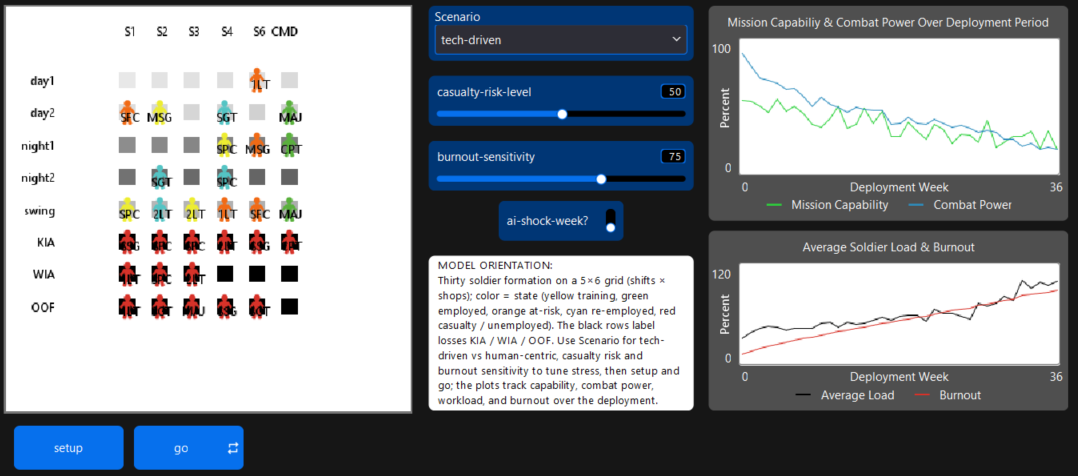
\includegraphics[width=0.82\textwidth]{model_snip1.png}

  \vspace{0.5em}
  \textbf{Human-Centric Support}\\[0.1em]
  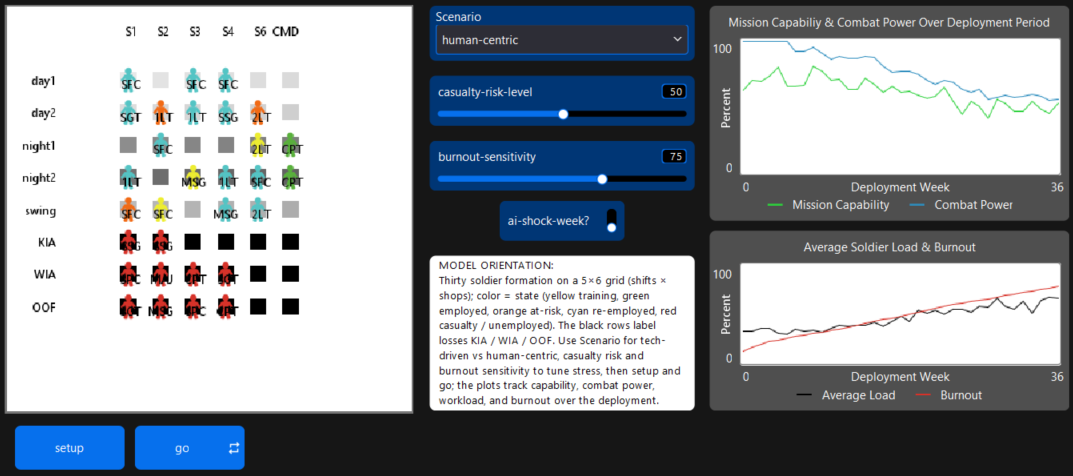
\includegraphics[width=0.82\textwidth]{model_snip2.png}

  \caption{Scenario comparison of system outputs (mission capability, combat power, load, and burnout) across the same deployment horizon.}
  \label{fig:scenario-comparison}
\end{figure}
% ---------------------------------------------------------------------------
\section{Reflection and Interpretation of the Model}

\textbf{Programmed components.} The model explicitly programs worker attributes, states, and transition rules: timed training completion, probabilistic movement from employed/re-employed to at-risk based on disruption risk and scenario pressure, conditional return from at-risk to in-training, and probabilistic casualties from active states. Scenario presets are also explicitly coded through different parameter values (automation pressure, human-loop effect, training-seat pressure, and AI capability growth), while system outputs are computed each tick from state counts and survivor conditions.

\textbf{Emergent system-level pattern.} The key emergent pattern is a workload-burnout feedback: as casualties and retraining temporarily reduce the active workforce, remaining workers absorb more load, which increases burnout; higher burnout then degrades recovery pace and system performance over time. This coupling is not a single hard-coded “collapse rule,” but a repeated result of local transitions and redistribution.

\textbf{Scenario differences.} Under Tech-Driven Automation, workers generally move into at-risk status more often, staffing volatility is higher, and capability trajectories tend to dip earlier or more sharply when losses accumulate. Under Human-Centric Support, the same model structure produces slower disruption flow, steadier re-employment, and smoother mission and burnout trends. In short, the scenarios differ mainly by support and pressure settings, and those programmed differences produce distinct aggregate behavior at the system level.

\textbf{Strengths.} The model is compact, inspectable, and maps cleanly onto the assignment: workers only, scenario-level policy, multiple states, mixed transition types (timed, probabilistic, conditional), and several aggregate outputs.

\textbf{Limitations.} (1) \textbf{Stylized calibration:} parameters are chosen for pedagogical contrast, not empirical Army or labor-market estimation. (2) \textbf{Homogeneous time step:} one week per tick abstracts away intra-week dynamics. (3) \textbf{Command column} is partly insulated from some transitions, which simplifies the grid but is a modeling choice made because decision makers charged with the survival of soldiers are the least likely to face AI disruption. 

% ---------------------------------------------------------------------------
\section*{AI Use Appendix}

\textbf{Tool(s) used:} Cursor and ChatGPT.

\textbf{Representative prompts (paraphrase):}
\begin{itemize}[leftmargin=*]
  \item Outline a compact NetLogo workforce model with 25--30 agents, explicit states, and two scenarios.
  \item Help map a deployed BDE HQ staff to labor-market concepts (task profile, behavioral trait, AI disruption risk, states, outputs).
  \item Debug NetLogo issues in iterative development (widget-variable wiring, duplicate globals, transition formulas, and plotting behavior).
  \item Refine memo structure and wording to align with the CO1 rubric sections and required interpretation points.
\end{itemize}

\textbf{What was accepted, revised, or rejected:}
\begin{itemize}[leftmargin=*]
  \item \textbf{Accepted (with edits):} initial state/transition scaffolding, scenario framing, and draft memo.
  \item \textbf{Revised manually:} transition probabilities, metric weights, casualty/burnout-load coupling, scenario parameter values, visualization notes, and final narrative tone.
  \item \textbf{Rejected:} suggestions that conflicted with NetLogo~7 behavior (e.g., duplicate widget globals), produced unstable dynamics, or reduced interpretability for the assignment context.
\end{itemize}

\textbf{Judgment statement:} There were many iterative prompts across planning, coding, debugging, and writing, too numerous to list individually. AI tools contributed substantially to draft code and memo text, while final model behavior, refinement, error correction, and submission framing were edited manually by the author.

\end{document}
